% T4_Equilibrium.pdf -- Cvičení: podmínky rovnováhy
\section{Cvičení: Podmínky rovnováhy}
\strana{T4-1}

\begin{priklad}[Příklad 1]
\begin{center}
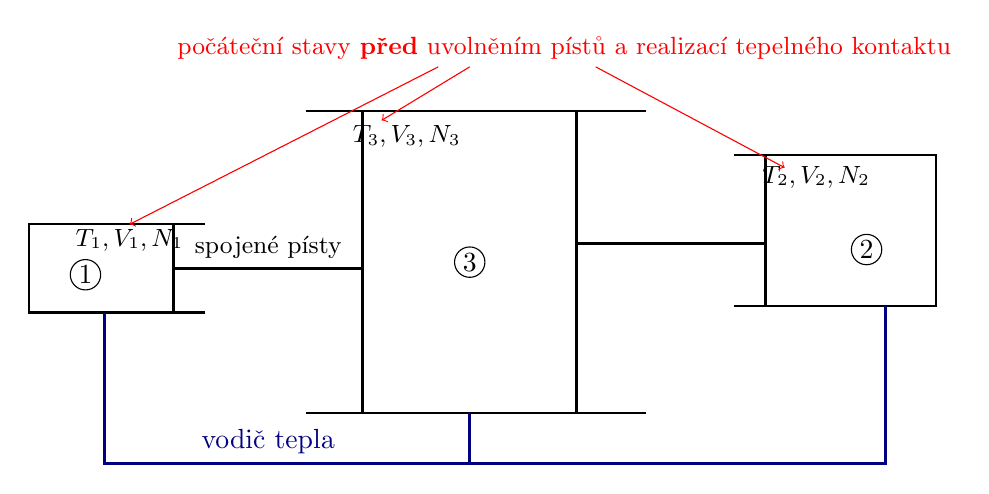
\begin{tikzpicture}[scale=0.8]
  % válec 1
  \draw[thick] (2.8,3.2) -- (0,3.2) -- (0,1.8) -- (2.8,1.8);
  \draw[very thick] (2.3,1.8) -- (2.3,3.2);
  \node[draw,circle,inner sep=1pt] at (0.9,2.4) {1};
  \node[font=\small] at (1.6,2.95) {$T_1,V_1,N_1$};
  % tyč 1-3
  \draw[very thick] (2.3,2.5) -- (5.3,2.5);
  \node[above,font=\small] at (3.8,2.5) {spojené písty};
  % válec 3
  \draw[thick] (4.4,5) -- (9.8,5);
  \draw[thick] (4.4,0.2) -- (9.8,0.2);
  \draw[very thick] (5.3,0.2) -- (5.3,5);
  \draw[very thick] (8.7,0.2) -- (8.7,5);
  \node[draw,circle,inner sep=1pt] at (7,2.6) {3};
  \node[font=\small] at (6,4.6) {$T_3,V_3,N_3$};
  % tyč 3-2
  \draw[very thick] (8.7,2.9) -- (11.7,2.9);
  % válec 2
  \draw[thick] (11.2,1.9) -- (14.4,1.9) -- (14.4,4.3) -- (11.2,4.3);
  \draw[very thick] (11.7,1.9) -- (11.7,4.3);
  \node[draw,circle,inner sep=1pt] at (13.3,2.8) {2};
  \node[font=\small] at (12.5,3.95) {$T_2,V_2,N_2$};
  % vodič tepla
  \draw[NavyBlue,very thick] (1.2,1.8) -- (1.2,-0.6) -- (13.6,-0.6) -- (13.6,1.9);
  \draw[NavyBlue,very thick] (7,0.2) -- (7,-0.6);
  \node[NavyBlue,above] at (3.8,-0.6) {\uv{vodič tepla}};
  % poznámka
  \node[Red,align=center,font=\small] at (8.5,6) {počáteční stavy \textbf{před} uvolněním pístů a realizací tepelného kontaktu};
  \draw[Red,->] (6.5,5.7) -- (1.6,3.2);
  \draw[Red,->] (7,5.7) -- (5.6,4.85);
  \draw[Red,->] (9,5.7) -- (12,4.1);
\end{tikzpicture}
\end{center}
Plyny ve válcích 1, 2, 3 si mohou vyměňovat teplo a prostřednictvím spojených pístů na sebe konat práci. Poměr ploch pístů je $A_1 : A_2 : A_3 = 1 : 2 : 3$. Najděte poměry tlaků v jednotlivých válcích.
\end{priklad}

\begin{enumerate}[label=\arabic*),font=\color{NavyBlue}]\color{NavyBlue}
  \item najděte $\dd S = \dd\left(\sum_{i=1}^3 S\right)$ pro entropickou FR obecného systému se třemi podsystémy
  \item identifikujte vazby a vyjádřete je v dif.\ tvaru:
  \begin{enumerate}[label=\roman*)]
    \item $U = \sum U_i = $ konst \quad $\Rightarrow$ \quad $\dd U_1 + \dd U_2 + \dd U_3 = 0$
    \item vazby na objemy -- kolik jich je a jaké?
  \end{enumerate}
  \item dosaďte vazby do $\dd S$ a vyjádřete $\dd S$ pouze pomocí nezávislých diferenciálů \\
  $\Rightarrow$ z $\dd S = 0$ identifikujte podmínky rovnováhy (pro každý nezávislý diferenciál dostanete jednu)
\end{enumerate}

\textcolor{NavyBlue}{
\underline{Pozn:} Získané podmínky rovnováhy,
\begin{align*}
  T_1 = T_2 = T_3 \quad &\Leftrightarrow\quad T_1(U_1,V_1,N_1) = T_2(U_2,V_2,N_2) = T_3(U_3,V_3,N_3) \\
  p_1 = \alpha p_2 = \beta p_3 \quad &\Leftrightarrow\quad p_1(U_1,V_1,N_1) = \alpha p_2(U_2,V_2,N_2) = \beta p_3(U_3,V_3,N_3)
\end{align*}
spolu s vazbami \quad $U_1 + U_2 + U_3 = U$ \\
\hspace*{3cm} $f_i(V_1,V_2,V_3) = 0 \qquad i = 1,\dots,?$ \\
jsou \underline{rovnice pro rovnovážné $U_{1,2,3}$ \& $V_{1,2,3}$} (viz postulát 2)
}

%----------------------------------------------------------------------
\strana{T4-2}
\begin{priklad}[Příklad 2: Mechanická rovnováha bez tepelného kontaktu]
\begin{center}
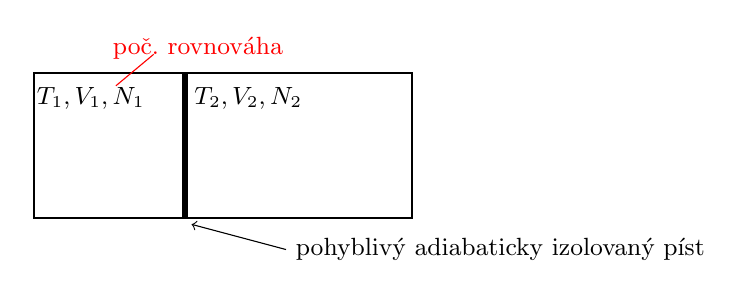
\begin{tikzpicture}[scale=0.8]
  \draw[thick] (0,0) rectangle (6,2.3);
  \draw[line width=2pt] (2.4,0) -- (2.4,2.3);
  \node[font=\small] at (0.9,1.9) {$T_1,V_1,N_1$};
  \node[font=\small] at (3.4,1.9) {$T_2,V_2,N_2$};
  \node[Red,font=\small] at (2.6,2.7) {poč.\ rovnováha};
  \draw[Red] (1.9,2.6) -- (1.3,2.1);
  \draw[->] (4,-0.5) node[right,font=\small] {pohyblivý adiabaticky izolovaný píst} -- (2.5,-0.1);
\end{tikzpicture}
\end{center}
Plyny ve dvou komorách jsou ve svých rovnovážných stavech. Uvolníme píst, ale nesejmeme adiabatickou izolaci. Jaká se ustaví rovnováha?
\end{priklad}

\color{NavyBlue}
\begin{itemize}
  \item $\dd N_i = 0$
  \item $\dd S = \dfrac{1}{T_1}\dd U_1 + \dfrac{p_1}{T_1}\dd V_1 + \dfrac{1}{T_2}\dd U_2 + \dfrac{p_2}{T_2}\dd V_2$
  \item \underline{vazby:} \quad $\bullet$ $V_1 + V_2 = V \ \Rightarrow\ \dd V_2 = -\dd V_1$ \\
  \hspace*{1.8cm} $\bullet$ energie se mění pouze prací $\Rightarrow$ $\dd U_i$ nejsou nezávislé na $\dd V_i$:
  \[ \dd U_i = -p_i\,\dd V_i \]
\end{itemize}
\[
  \Rightarrow\ \dd S = \underbrace{-\frac{p_1}{T_1}\dd V_1}_{\frac{1}{T_1}\dd U_1} + \left(\frac{p_1}{T_1} - \frac{p_2}{T_2}\right)\dd V_1 + \underbrace{\frac{p_2}{T_2}\dd V_1}_{\frac{1}{T_2}\dd U_2} \equiv 0
\]
$\Rightarrow$ podmínky rovnováhy nic nedávají, $\dd S\equiv 0$ \\
\quad (jistě, jedná se o vratný proces, nedochází k výměně tepla)
\begin{itemize}
  \item podmínku rovnováhy dostáváme jedinou ze (zatím) opomenuté vazby
\end{itemize}
\[
  U_1 + U_2 = U \ \Rightarrow\ 0 = \dd U_1 + \dd U_2 = -p_1\,\dd V_1 - p_2\,\dd V_2 = (p_2 - p_1)\,\dd V_1
\]
\[
  \Rightarrow\ \vzorec{p_1 = p_2} \text{ v rovnováze platí}
\]
\[
  \Leftrightarrow\ p_1(U_1,V_1,N_1) = p_2(U - U_1, V - V_1, N_2)
\]
\begin{itemize}
  \item 1 rce pro neznámé $U_1, V_1$ ovšem nestačí
  \item aby se ustavila rovnováha, je třeba disipace; její míra v jednotlivých komorách určuje rozdělení $U_1 + U_2 = U \Rightarrow T_1, T_2$
\end{itemize}
\color{black}

%----------------------------------------------------------------------
\strana{T4-3}
\begin{priklad}[Příklad 3: Rovnováha při výměně částic]
Dvoukomponentní systém popsaný fund.\ rovnicí
\[
  S = NA + NR\log\big(U^{3/2}VN^{-5/2}\big) - R\sum_{i=1}^2 N_i\log\frac{N_i}{N}\,; \qquad N = N_1 + N_2
\]
se nachází ve dvou oddělených komorách. Počáteční teploty, objemy a počty částic jsou
\[
  T_\alpha,\ V_\alpha = \tfrac12 V,\ N_{1\alpha}^0,\ N_{2\alpha}^0\,; \qquad \alpha = L, R \quad \text{(levá/pravá komora)}
\]
$\Rightarrow N_1 = N_{1L}^0 + N_{1R}^0$, \ $N_2 = N_{2L}^0 + N_{2R}^0$ \ jsou celkové počty molů částic typu 1 resp.\ 2.

Nyní z přepážky sejmeme izolaci tak, že začne propouštět teplo a částice typu 1 (semi-permeabilní stěna). Jaká rovnováha se ustaví ($T_\alpha^f, N_{1\alpha}^f, N_{2\alpha}^f$; objemy se nemění)?
\end{priklad}

\begin{enumerate}[label=\arabic*),font=\color{NavyBlue}]\color{NavyBlue}
  \item $\dd S = 0$ pomocí diferenciálů měnících se proměnných
  \item vazby $\Rightarrow$ $\dd S = 0$ pouze pomocí diferenciálů nezávislých proměnných
  \[ \Rightarrow\ \dd S = \sum_i\underbrace{(\quad\ )}_{=0}\dd X_i \]
  \item spolu s vazbami dostáváme potřebný počet rovnic pro neznámé $T_L^f, T_R^f$ \& $N_{1L}, N_{1R}$ ($N_{2\alpha}$ se nemění)
\end{enumerate}

\begin{center}\color{Red}
$\vzorec{T_\alpha^f = T_f = \dfrac{N_L^0T_L + N_R^0T_R}{N}}\,; \qquad N_\alpha^0 = N_{1\alpha}^0 + N_{2\alpha}^0, \quad N = N_L^0 + N_R^0$

\medskip
$\vzorec{N_{1L} = N_{1R} = \tfrac12 N_1}$ \quad \dots\ odpovídá také rovnosti \underline{parciálních tlaků} (systém je 2-komp.\ id.\ plyn)
\end{center}

